\documentclass{article}

\usepackage[brazil]{babel}
\usepackage[T1]{fontenc}
\usepackage[a4paper, margin=1.5cm]{geometry}
\usepackage[colorlinks, urlcolor=blue, citecolor=red]{hyperref}
\usepackage[utf8]{inputenc}
\usepackage{enumitem, graphicx}

\title{\textbf{Exemplo de poda $\alpha$-$\beta$ e função heurística para damas}}
\author{Emmanuel Podestá Jr., Gustavo Zambonin\thanks{
    \texttt{\{emmanuel.podesta,gustavo.zambonin\}@grad.ufsc.br}} \\
\small {Inteligência Artificial (UFSC -- INE5430)} \vspace{-5mm}}
\date{}

\begin{document}

\maketitle

\begin{enumerate}[label=\textbf{\arabic*})]

    \item Em anexo ao final do documento, a árvore resolvida a partir do
    algoritmo de poda. Para os nodos folha, $\alpha$ e $\beta$ não foram
    computados para que a imagem não ficasse confusa; locais marcados com
    um asterisco (*) são passíveis de poda caso existissem outros filhos.

    \begin{figure}
        \centering
        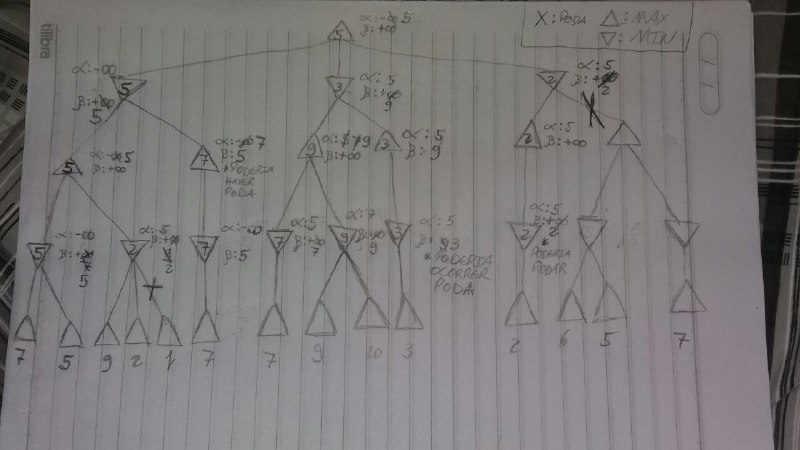
\includegraphics[width=1\textwidth]{arvore.jpg}
    \end{figure}

    \item Considerando um jogo de damas usual e observando um modelo de grafo
    convencional, que mapeia estados do tabuleiro para nodos e jogadas válidas
    conectando-os como arestas, é possível observar que tal árvore resultante
    impossibilitará o uso de uma função utilidade apenas, por conta do seu
    vasto número de possibilidades para jogadas.

    Analisando as regras do jogo, alguns tópicos foram escolhidos de modo a
    diferenciar um tabuleiro que representa uma boa jogada. Estes podem ser
    utilizados para ambos os tipos de funções.

    \begin{itemize}

        \item É necessário normalizar o valor do tabuleiro em relação ao
        jogador humano, então pode-se decrementar da pontuação deste o valor
        obtido pela análise das peças do jogador computacional.

        \item O número de `'damas`' do jogador deve influenciar mais no valor
        final do tabuleiro do que peças normais, visto que é mais difícil
        obtê-las e sua capacidade de movimentação e ataque são melhoradas.

        \item O número de peças no tabuleiro é um fator a ser considerado,
        visto que é muito mais difícil vencer um jogo se suas peças estão
        cercadas por outras de cor diferente.

        \item As possibilidades de ataque de peças normais e `'damas`' devem
        ser consideradas, de modo que o algoritmo deve verificar se existem
        movimentos que possam remover uma ou mais peças do adversário; porém,
        tais verificações serão mais custosas em virtude do incremento da
        procura em profundidade para considerar ataques duplos ou triplos.

    \end{itemize}

    Note que tais análises são extremamente ingênuas; para produzir um
    jogador computacional hábil, recursos como a pré-computação de valores
    para estados de tabuleiros específicos, na forma de bancos de dados;
    grandes listagens de movimentos de abertura, para maximizar a chance de
    boas jogadas desde o começo; e otimizações como tabelas de
    transposição\footnote{tabelas que guardam estados de tabuleiro que são
    iguais e alcançáveis por um grande número de jogadas diferentes;
    ou seja, caso uma jogada já tenha sido descartada e um tabuleiro similar
    aparece novamente, uma consulta nesta tabela pode acelerar a procura de
    possibilidades no algoritmo, descartando este tabuleiro.} podem ser
    inseridos no algoritmo para que seu conhecimento seja aumentado.
    Todos estes exemplos foram aplicados no jogador \textit{Chinook}
    \cite{Schaeffer1989}.

\end{enumerate}

\bibliography{ine5430_t1}
\bibliographystyle{plain}

\end{document}